\documentclass[number]{ximera}

%\usepackage{tikz}

\renewcommand{\theenumi}{\arabic{enumi}.}


% set font encoding for PDFLaTeX, XeLaTeX, or LuaTeX
\usepackage{ifxetex,ifluatex}
\newif\ifxetexorluatex
\ifxetex
  \xetexorluatextrue
\else
  \ifluatex
    \xetexorluatextrue
  \else
    \xetexorluatexfalse
  \fi
\fi

\ifxetexorluatex
  \usepackage{fontspec}
\else
  \usepackage[T1]{fontenc}
  \usepackage[utf8]{inputenc}
  \usepackage{lmodern}
\fi

\usepackage{hyperref}


%My github password is ximera1
%My GeoGebra password is Ximera1

\title{Special Triangles}
\author{Univ. of Minnesota MathCEP}

\begin{document}

\begin{abstract}
Recall that a triangle has three angles that add up to $180^\circ$.
A right triangle is a triangle that has one $90^\circ$ angle; the side opposite this angle is called the hypotenuse.
In this activity, we will look at two special cases of right triangles: when the remaining two angles are each $45^\circ$, and when the remaining two angles are $30^\circ$ and $60^\circ$.
Our goal is to determine the lengths of the legs of these triangles when the hypotenuse is 1.
\end{abstract}

\maketitle

For the $45^\circ-45^\circ-90^\circ$ triangle, (the isosceles right triangle), there are two legs of length $a$
and the hypotenuse of length 1.
\begin{image}
\begin{tikzpicture}[scale=2]
		\draw (0,0) -- node[below] {$a$} (2,0) -- node[above right] {$1$} (0,2) -- node[left] {$a$} (0,0) -- cycle;
		\draw (0,0.2) -- (0.2,0.2) -- (0.2,0);
		\node at (1.6,0.15) {$45^\circ$};	
		\node at (0.2,1.55) {$45^\circ$};	
\end{tikzpicture}			
%\caption{A $45^\circ-45^\circ-90^\circ$ triangle.}
\end{image}


\begin{problem}
Use the Pythagorean Theorem to write an equation relating the lengths of the sides of the triangle: $\answer{a}^2+\answer{a}^2=\answer{1}^2$.
\begin{hint}
In a right triangle with sides lengths $a$ and $b$ and hypotenuse $c$, the Pythagorean Theorem states that $a^2+b^2=c^2$.
\end{hint}

\end{problem}

\begin{problem}
Solve the equation for $a = \answer{\frac{\sqrt{2}}{2}}$.
\begin{hint}
How can you write $a^2+a^2$ as one term?
\end{hint}
\end{problem}

\begin{problem}
In summary, a $45^\circ-45^\circ-90^\circ$ triangle has:

base $=\answer{\frac{\sqrt{2}}{2}}$

height $=\answer{\frac{\sqrt{2}}{2}}$

hypotenouse $=\answer{1}$
\end{problem}

To find the lengths of the legs of the $30^\circ-60^\circ-90^\circ$ triangle, begin with an equilateral triangle, all of whose sides are length 1. 
Recall that in an equilateral triangle, all three angles are equal to $60^\circ$.
One possible approach to solving for the side lengths is the following:

\begin{image}
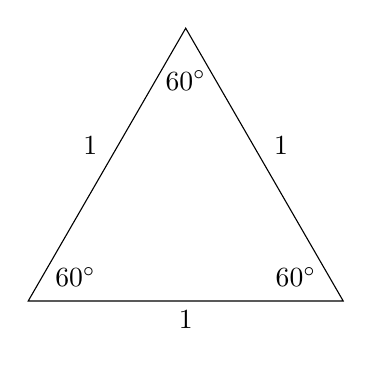
\begin{tikzpicture}[scale=2]
		\draw (0,0) -- node[below] {$1$} (2,0) -- node[above right] {$1$} (1,1.732) -- node[above left] {$1$} (0,0) -- cycle;
		\node at (0.3,0.15) {$60^\circ$};		
		\node at (1,1.4) {$60^\circ$};		
		\node at (1.7,0.15) {$60^\circ$};		
\end{tikzpicture}			
%\caption{An equilateral triangle.}
\end{image}

\begin{problem}
From the top vertex, draw a line segment perpendicular to the bottom side, cutting the original triangle into two congruent triangles.
In an equilateral triangle, this line segment is called a perpendicuar bisector, a median, and an altitude.

The length of each half of the bottom side is $b=\answer{\frac{1}{2}}$.
\end{problem}

\begin{problem}
Find all of the angles in the new triangles determined by the perpendicular bisector you drew in the previous problem.

Smallest $\measuredangle = \answer{30}^\circ$

Second smallest $\measuredangle = \answer{60}^\circ$

Largest $\measuredangle = \answer{90}^\circ$

\begin{hint}
The angles add up to $180^\circ$.
\end{hint}
\end{problem}

\begin{problem}
Label the length of the altitude $h$, and use the Pythagorean theorem to write an equation involving $h$:
\begin{freeResponse} %I can't think of a way to format the answer that doesn't involve giving too much of a hint
\end{freeResponse}
\begin{hint} In a right triangle with sides lengths $a$ and $b$ and hypotenuse $c$, the Pythagorean Theorem states that $a^2+b^2=c^2$.\end{hint}
\end{problem}


\begin{problem}
Solve the equation for $h$ in the expression you wrote above: 

$h = \answer{\frac{\sqrt{3}}{2}}$
\end{problem}

\begin{problem}
In summary, a $30^\circ-60^\circ-90^\circ$ triangle has:

base $=\answer{\frac{1}{2}}$

height $=\answer{\frac{\sqrt{3}}{2}}$

hypotenouse $=\answer{1}$
\end{problem}

\begin{exercise} Draw the 45-45-90 triangle in as many orientations as possible, keeping the legs either horizontal or vertical. How many are there? $\answer{4}$
\begin{hint}
You can rotate and reflect the triangle.
\end{hint}
\end{exercise}

\begin{exercise} Draw the 30-60-90 triangle in as many orientations as possible, keeping the legs either horizontal or vertical. How many are there? $\answer{8}$
\begin{hint}
Do you expect this number to be the same as in the 45-45-90 case?
\end{hint}
\end{exercise}

\end{document}

